\documentclass[prl,twocolumn,superscriptaddress]{revtex4-1}
\pdfoutput=1
\usepackage[letterpaper,top=1.45cm,bottom=1.65cm,left=2cm,right=2cm]{geometry}
\usepackage{amssymb,amsmath,amsthm,graphicx,mathptmx}
\usepackage{subfigure}
\usepackage{graphics, color}
\usepackage{latexsym}
\usepackage{bm}
\usepackage{epsfig}
\usepackage{multirow,tabularx}
\usepackage[colorlinks=true,linktocpage=true,linkcolor=blue,citecolor=blue]{hyperref}
\usepackage[abs]{overpic}

\usepackage{fancyhdr}
\fancyhf{}
\cfoot{\thepage}
\renewcommand{\headrulewidth}{0pt}
\pagestyle{fancy}
\fancypagestyle{plain}

\setlength{\parskip}{0cm}

\newcommand{\PRLsection}[1]{\emph{#1.---}}

\newcommand{\ToDo}[1]{\textbf{\textsf !#1!}}
\newcommand{\TF}{\mathrm{TF}}  %TF
\newcolumntype{Y}{>{\centering\arraybackslash}X}

\newtheorem{theorem}{Theorem}[section]
\newtheorem{example}[theorem]{Example}
\newtheorem{definition}[theorem]{Definition}
\newtheorem{exercise}[theorem]{Exercise}
\newtheorem{proposition}[theorem]{Proposition}
\newtheorem{note}[theorem]{Note}
\newtheorem{lemma}[theorem]{Lemma}
\newtheorem{corollary}[theorem]{Corollary}
\newtheorem{unusedproblem}[theorem]{unused Problem}
\newtheorem{question}[theorem]{Question}
\newtheorem{project}[theorem]{Project}
\newtheorem{problem}[theorem]{Problem}
\newtheorem{conjecture}[theorem]{Conjecture}
\newtheorem{remark}[theorem]{Remark}


%%%%%%%%%%%%%%%%%%%%%%%%
% Document
%%%%%%%%%%%%%%%%%%%%%%%%
\begin{document}

\title{Compact Scalar Solitons as Holographic Heavy Ions}

\author{Hans Bantilan}
\email{h.bantilan@qmul.ac.uk}
\affiliation{School of Mathematical Sciences, Queen Mary University of London, Mile End Road, London E1 4NS, United Kingdom}
\affiliation{Centre for Research in String Theory, School of Physics and Astronomy, Queen Mary University of London, E1 4NS, UK}
\author{Thomas Helfer}
\email{thomashelfer@live.de}
\affiliation{Theoretical Particle Physics and Cosmology Group, Physics Department, Kings College London, Strand, London WC2R 2LS, United Kingdom}

\begin{abstract}

\end{abstract}

\maketitle

%-------------------------------------------------------
% Introduction
%-------------------------------------------------------
\PRLsection{Introduction}

\medskip

%-------------------------------------------------------
% Setup
%-------------------------------------------------------
\PRLsection{Setup}

\medskip

%-------------------------------------------------------
% Numerical Scheme
%-------------------------------------------------------
\PRLsection{Numerical Scheme}

\medskip

%-------------------------------------------------------
% Results
%-------------------------------------------------------
\PRLsection{Results}

\begin{figure}[t]
  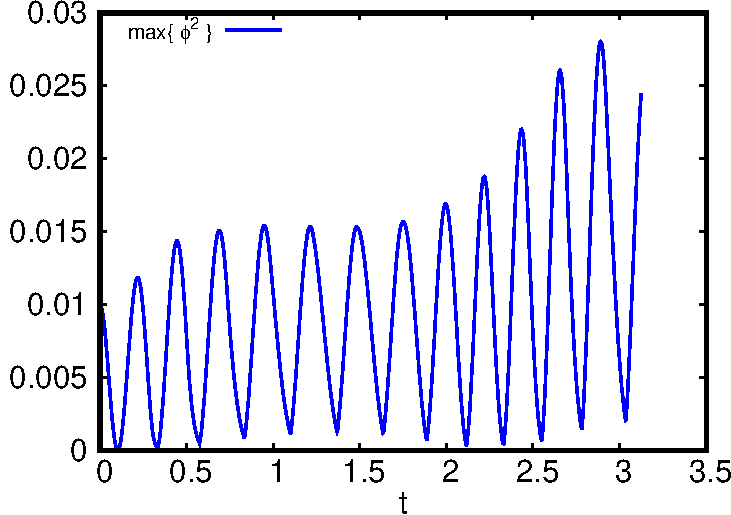
\includegraphics[width=\linewidth]{diagnostic-single.pdf}
                        {\caption{
                            The maximum of $\varphi^2$ for a single oscillaton in AdS, for a simulation generated from initial data with maximum scalar field amplitude $\left. \varphi_{max} \right|_{t=0}=0.1$. 
For this diagnostic, a constant envelope is a good indication of stability.
                        }\label{fig:diagnostic-single}}
\end{figure}

\begin{figure}[t]
  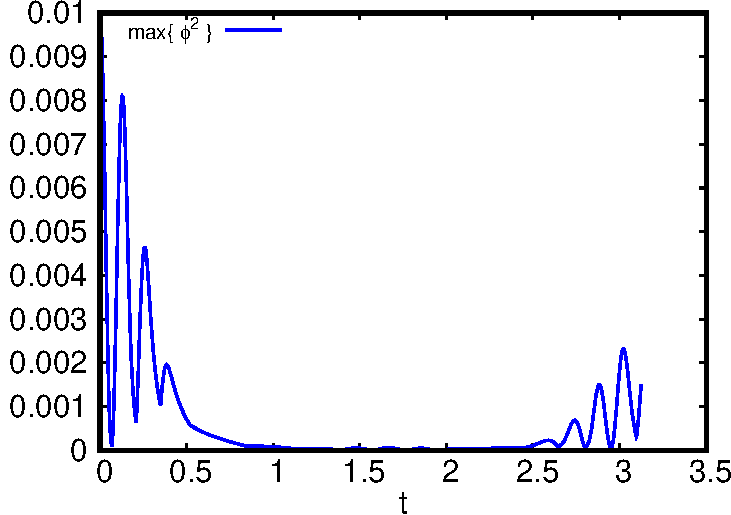
\includegraphics[width=\linewidth]{diagnostic-collision.pdf}
                        {\caption{
                            The maximum of $\varphi^2$ for the collision of two oscillatons in AdS, for a simulation generated from initial data with maximum scalar field amplitude $\left. \varphi_{max} \right|_{t=0}=0.1$. In this simulation, the collision does not result in black hole formation. The oscillatons propagate past each other and reform at antipodal points after a global time of $\pi$ with a diminished maximum amplitude of $\left. \varphi_{max} \right|_{t=\pi}=0.0388$.
                        }\label{fig:diagnostic-single}}
\end{figure}

\medskip

%-------------------------------------------------------
% Discussion
%-------------------------------------------------------
\PRLsection{Discussion}

\medskip

%-------------------------------------------------------
% Acknowledgements
%-------------------------------------------------------
\PRLsection{Acknowledgements}
Simulations were run on the {\bf Perseus} cluster at Princeton University and the {\bf MareNostrum}
cluster at the Barcelona Supercomputing Center.

\medskip

%-------------------------------------------------------
% Bibliography
%-------------------------------------------------------
%\bibliography{oscillaton}
\bibliographystyle{apsrev4-1}

\end{document}
